% !TeX spellcheck = zh_CN
% !BIB program = bibtex
\documentclass[aps,pre,12pt,preprint,%
	onecolumn,showpacs,showkeys,nofootinbib]{revtex4-1}
%UnlimitedFonts
	\def\hmmax{0}
	\def\bmmax{0}
%SVG
	\usepackage{svg}
%Tables
	\usepackage{array,booktabs,tabularx,multirow}
	\newcolumntype{C}[1]{>{\hsize=#1\hsize%
		\centering\arraybackslash}X}
%Math&Fonts
	\let\latexointop\ointop
	\usepackage{mathtools,amssymb,bm % basics
		,physics,siunitx,slashed % physics
		,esint,nicefrac,extarrows,mathrsfs % more symbols
		,calligra,romannum,dsfont,fourier-orns % nice fonts
		,eqnarray,resizegather,empheq % more envs
		,relsize,stackengine % utils
	}
%	\usepackage{amsthm}
	\usepackage[scr=esstix]{mathalfa}
	\usepackage[only,sslash]{stmaryrd}
	%DisplaySetup
	\newcommand*\bbox[1]{\fbox{\hspace{1em}\addstackgap[5pt]{#1}\hspace{1em}}}
	\empheqset{box=\bbox}
	\mathtoolsset{showonlyrefs}
%Utils
	%Legacy \oint
	\let\ointop\undefined
	\let\ointop\latexointop
	%Calligra
	\DeclareMathAlphabet{\mathcalligra}{T1}{calligra}{m}{n}
	\DeclareFontShape{T1}{calligra}{m}{n}{<->s*[2.2]callig15}{}
	%CosmeticTweaks
	\newcommand\inlineeqno{\stepcounter{equation}\ (\theequation)}
	\newcommand\scalemath[2]{\scalebox{#1}{\mbox{\ensuremath{\displaystyle #2}}}}
	\newcommand\raisemath[2]{\raisebox{#1\depth}{${#2}$}}
	\newfontfamily\signature{Vladimir Script}
	\newcommand{\newparagraph}{\pagebreak[3]
		\noindent\hfil%
		\raisebox{-4pt}[10pt][10pt]{\leafright~\qquad~\leafleft}%
		\par\nopagebreak%
	}
%CustomCmds
	%Brackets
	\DeclarePairedDelimiter\ave{\langle}{\rangle}
	\DeclarePairedDelimiterX\inprod[2]{\langle}{\rangle}{#1,#2}
	%Basics
	\newcommand{\mbb}[1]{\mathbb{#1}}
	\newcommand{\mrm}[1]{\mathrm{#1}}
	\newcommand{\mcal}[1]{\mathcal{#1}}
	\newcommand{\mscr}[1]{\mathscr{#1}}
	\newcommand{\tup}[1]{\textup{#1}}
	\newcommand{\mop}[1]{\operatorname{#1}}
	%Extras
	\newcommand{\scriptr}{\mathcalligra{r}\,}
	\newcommand{\rvector}{\pmb{\mathcalligra{r}}\,}
	\newcommand{\hodgedual}{\operatorname{\star}}
	\newcommand{\dual}{\ \xlongleftrightarrow{\ \textrm{dual}\ }\ }
	\newcommand{\idty}{\mathds{1}}
	\newcommand{\proj}[1]{\operatorname{%
		proj_{\mathit{#1}}}}
	\newcommand{\propsim}{\mathbin{\ensurestackMath{
		\stackunder[2pt]{\propto}{\sim}
	}}}
	\newcommand{\textbox}[1]{\fbox{#1}}
	\newcommand{\pdd}[1]{\operatorname{\partial_{\mathnormal{#1}}}}
	\newcommand{\cdd}{\operatorname{D}\!}
	\newcommand{\cdv}[1]{\operatorname{%
		\nabla_{\!\mathit{#1}\!}}}
	\newcommand{\ldv}[1]{\operatorname{%
		\mcal{L}_{\!\mathit{#1}\!}}}
	\newcommand{\ric}[1]{\operatorname{%
		Ric}\!\pqty{#1}}
%Hacks
	% physics.sty <texmf-dist/tex/latex/physics/>
	% USER: more spacing around Dirac's middle vert
	\newcommand{\xmiddle}[1]{\mspace{1mu}\middle#1\mspace{1mu}}
	\DeclareDocumentCommand\innerproduct{ s m g }
	{ % Inner product
		\IfBooleanTF{#1}
		{ % No resize
			\IfNoValueTF{#3}
			{\vphantom{#2}\left\langle\smash{#2}\xmiddle\vert\smash{#2}\right\rangle}
			{\vphantom{#2#3}\left\langle\smash{#2}\xmiddle\vert\smash{#3}\right\rangle}
		}
		{ % Auto resize
			\IfNoValueTF{#3}
			{\left\langle{#2}\xmiddle\vert{#2}\right\rangle}
			{\left\langle{#2}\xmiddle\vert{#3}\right\rangle}
		}
	}

%Miscellaneous
%	\newcommand{\tabindent}{\hspace{2em}}
	\newcommand{\naItl}{\tup{NaI\,(Tl)}}
	\newcommand{\perc}[1]{\SI{#1}{\percent}}
	\newcommand{\csAtom}{${}^{137}\mrm{Cs}$}
	\newcommand{\coAtom}{${}^{60}\mrm{Co}$}
	\newcommand{\rayleighNumber}{\mrm{Ra}}
\begin{document}
%Basic Data
	\title{%
	\texstringonly{\hfil\\[2\baselineskip]}
	\sf\LARGE%
		阴影法研究非线性热对流斑图%
	\texstringonly{\vspace{3ex}}}
	\author{\fangsong\large%
		Bryan%
	\vspace{2mm}}
	\affiliation{\it%
		北京大学物理学院~~学号:\normalfont 1500066666\,}
	\date{\today}
	\keywords{耗散结构理论\quad Rayleigh–Bénard对流\quad 非线性物理}
	\email{masked_email_please_contact@github.com}

\begin{abstract}
\vspace{10mm}
\begin{spacing}{1.5}\normalsize
\setlength{\parskip}{.3\baselineskip}
%	200—300字,
%	说明用什么方法做了什么事,
%	由此得到什么结果和结论,
%	有何意义.
%	不用缩略词,不用第一人称.
%%%%%%%%%%%%%%%%%%%%%%%%%%%%%%%%
	本实验通过观察Rayleigh–Bénard对流现象的产生、发展和演化过程,了解了耗散结构理论及非线性动力学的基本内容。
	
	具体而言,实验中通过控制 \SI{2}{\mm}, \SI{4}{\mm} 薄层去离子水的上下表面温差,观察到了非线性对流从无到有、从稳定有序到失稳湍流的转变过程,并借此图像定性地分析了系统相应结构的特征。
\end{spacing}
\end{abstract}

\maketitle
\thispagestyle{titlepagestyle}

%%  课程实验报告应假定读者既不是已知全部实验细节的指导教师,也不是缺少专业知识的公众,而是同领域的实验研究者,或审稿人. 不能要求读者要在读过课程讲义后才能读懂课程实验报告.
%%  凡不是自己独立思考得到的内容都应该引参考文献. 不能大段引用同一参考文献. 对复杂问题,应该优先考虑引用参考文献得到结果. 对简单一些的问题才鼓励独立思考.
\section{引言}
%%	研究论文引言一般包含以下内容:
%%	(1)所研究领域背景和现状;
%%	(2)有待研究的问题;
%%	(3)本研究的目的、主要内容和结果;
%%	(4)结果的意义.\par
%%	在写实验报告的引言时,同学可以假想自己是第一个做类似研究的人.\par
%%	引言一定要切合报告正文,不能漫无目的地介绍背景. 要快速地将读者引导到报告主题上,并作较深入的讨论.\par
%%	引言篇幅可以在较大范围内变化,但最长不应超过报告文字篇幅的1/3.\par
%%	引言撰写可以参考实验讲义,可以复述,但不能复制讲义上的任何一句话.\par
%%%%%%%%%%%%%%%%%%%%%%%%%%%%%%%
%\vspace{-1ex}
	自然界中存在丰富的自组织现象,即由局域的相互作用、从无序初态出发,自发地产生出更大尺度上的有序结构。常见的例子有热对流结构(\textit{如大气环流}),结晶过程(\textit{如冰晶形成}),化学振荡(\textit{如碘钟} \cite{lambert1984iodine}),生命过程(\textit{大至进化,小至蛋白质的合成与折叠})等等。从对称性的角度上看,自组织现象往往与所谓\mbox{\textit{自发对称性破缺}}密切相关;这一观点在理论物理当中十分关键,它描述了统一理论到各种相互作用的过渡,如电弱(electroweak)理论到电、弱相互作用的分离过程。
	
	由于考虑的往往是开放系统,上述现象与热力学第二定律暗示的无序演化恰好相反。虽说上述自组织现象往往可以通过具体的动力学加以分析,人们更希望以一种统一的语言对上述规律加以描述。正是基于此,Ilya Prigogine于上世纪60年代发展出了耗散结构(dissipative structure)理论 \cite{prigogine1978time}, 这一工作于1977年获得Nobel化学奖。
	
	据 \cite{textbook}, 耗散结构理论表明,当开放系统偏离平衡达一定程度时,系统将会出现分岔行为,此后系统将离开原先无序的热力学分支,发生突变进入到一个全新的稳定有序状态,此即耗散结构;若将系统拉开到离平衡态更远的地方,系统可能出现更多新的稳定有序状态。理论指出,系统从无序状态过渡到耗散结构有两个必要条件:
	\begin{enumerate}[noitemsep,label=\arabic*.]
	\item \textbf{系统必须开放},与外界进行物质或能量交换;
	\item \textbf{系统必须远离平衡},突破近平衡的线性动力学而采用非线性动力学。
	\end{enumerate}
	
	动力学上,在系统的非线性效应很小时,系统内部出现的随机涨落会衰减,但当系统的非线性效应不可忽略时,系统内部的产生的随机涨落会会逐渐变大,自组织后形成稳定的耗散结构。
		
	本实验观察的Rayleigh–Bénard对流正是耗散结构的一个具体实例。对流由薄液层的上下温差驱动,在突破静态的稳定临界条件时出现;此时通过阴影法可观察到有序的斑图。当温差过大时,耗散结构崩溃而被湍流所取代。本实验通过观察对流版图的形成与演化,以初步了解非线性动力学的基本特征,同时检验耗散结构的上述特性。
\clearpage
\section{理论}
\vspace{-1\baselineskip}
\setlength{\jot}{0pt}
	\begin{figure}[!ht]
		\centering
		\includesvg[width=.5\linewidth]{img/ConvectionCells.svg}
		\par\vspace{.5\baselineskip}
		\caption[Rayleigh–Bénard对流图示]{%
			\tup{Rayleigh–Bénard}对流图示,选自 \cite{wiki:convection}. %
		}
		\label{fig:convectionSketch}
%		\vspace{-1\baselineskip}
	\end{figure}
	
	Rayleigh–Bénard对流的基本结构如图;参考 \cite{textbook}, 基于Navier–Stokes可给出薄液层的运动方程;将其无量纲化后可得参量Rayleigh数:
	\begin{equation}
		\rayleighNumber
		= \frac{g\alpha d^3\Delta T}{\kappa\gamma}
		\propto d^3\Delta T
	\end{equation}
	其中$\alpha,\gamma,\kappa$分别为流体的热膨胀系数、粘度和热导率,$g$为重力加速度,$d$为薄液层厚度,$\Delta T$为温差。
	
	不难验证方程总有定常解,此时流速场$\vb{V}\equiv 0$. 采用线性稳定分析方法可考察上述静态解的稳定性;考虑$z$方向上的初始微扰:
	\begin{equation}
		u_z = A(z)\,e^{i\vb{k}\cdot\vb{r}_{\sslash}}\,e^{st},\quad
		\norm{\vb{k}} = \alpha,\quad
		\vb{r}_{\sslash} \cdot \hat{\vb{z}} = 0
	\end{equation}
	这里假定微扰为$xy$平面内的行波($e^{i\vb{k}\cdot\vb{r}_{\sslash}}$);带入方程略去非线性项(高阶小量),由$\Re s$可得微扰的稳定性,由此得到静态解失稳的临界参数。结合数值计算,可得对Rayleigh数$\rayleighNumber$, 有临界参量:
	\begin{equation}
		R_c \simeq 1707.75
	\end{equation}
	
	$\rayleighNumber > R_c$时,线性项不足以维持静态稳定,此时$\Re s > 0$, 扰动按指数$e^{st}$规律放大,非线性项将发挥重要作用。对本例而言,$\rayleighNumber \gtrsim R_c$时,由于非线性项的贡献,系统形成稳定的对流斑图;据 \cite{textbook}, 其稳态解可由弱非线性情况下的多尺度分析给出。$\rayleighNumber$显著大于$R_c$时,稳定的对流结构不足以支撑能量传递,此时对流失稳,体现为湍流。
%	\begin{figure}[!ht]
%		\centering
%		%\includeegraphics[width=.5\linewidth]{img/Klein-Nishina_distribution.png}
%		\caption[Compton散射的微分截面]{%
%			\tup{Compton}散射的微分散射截面,选自 \cite{wiki:klein-nishina}. %
%		}
%		\label{fig:ComptonSection}
%		\begin{explain}\footnotesize
%			\hspace{2em}图中圆周上标记的坐标为散射角$\theta/\si{\deg}\in\bqty{0,180}$, 不同$E_\gamma$对应的微分截面相对大小以不同颜色的曲线标记。可见,当$E_\gamma\ll m_e c^2$时(图中蓝线)微分截面与经典的\tup{Thomson}散射一致,正比于$\frac{1 + \cos^2\theta}{2}$, 微分截面关于$\theta = \frac{\pi}{2}$对称,即向前、向后散射截面对称。增大$E_\gamma$, 散射截面减小,且向前、向后散射截面不再对称;向前散射的概率大于向后散射。
%		\end{explain}
%		\vspace{-1\baselineskip}
%	\end{figure}
\restorejot
%%%%%%%%%%%%%%%%%%%%%
\section{实验装置}
\vspace{-.5\baselineskip}
	\begin{figure}[!ht]
		\centering
		\hspace{-.1\linewidth}%
		\includesvg[width=.45\linewidth]{img/Apparatus.svg}
		\par\vspace{.5\baselineskip}
		\caption[阴影法观察对流斑图的实验装置]{%
			阴影法观察对流斑图的实验装置,参见 \cite{textbook}. %
		}
		\label{fig:apparatus}
%		\vspace{-1\baselineskip}
	\end{figure}
	实验装置如图所示。实验观察的对流液层$d = \SI{2}{\mm}, \SI{4}{\mm}$, 上、下表面均选用高热导率界面以使温度均匀分布。上表面水冷降温,采用透明介质以便于观察;底面为硅胶片加热的铜盘,表面光洁以作为反射面。
	
	实验通过阴影法观察对流斑图,以准平行光正入射液层,考察经底面铜盘反射的光线之光强分布。光强分布直接反映液层的折射率分布;据Fermat原理,光线向高折射率区域偏折,即液层中的高折射率区域将会聚光线而形成亮区。进一步,高折射率对应高密度,即对流中的冷水下降区域,参见图 \ref{fig:convectionSketch}. 
\clearpage
\section{结果与分析}
%	实验结果应尽量以图表的形式给出. 每一个图表都应该是完整的,即阅读图表时可以不必依赖正文.\par
%	依自己意愿,实验结果和对结果的分析讨论既可分为两节也可合在一节.\par
%
%	每个图一般包含:图名、轴名、轴、刻度、标尺、数据点、曲线、图例、标注和图注等部分. 应尽量让读者不看正文就能基本理解图的含意.\par
%	逐点测量得到的函数关系要同时用表格和图给出. 需要作比较的多条曲线要画在同一图上.\par
%	为避免读者在图表和正文间反复跳跃阅读,在正文中也要对图表作必要的说明.\par
%
%	对于预料之外的实验结果,必须首先小心证明其可靠性.读者只有在相信你的实验结果时才愿意花时间看你的分析.\par
%	必须用文字归纳整理出正式的实验结果或结论.可信的实验结果是课程报告最重要的内容.作为一个实验物理工作者,分析解释出错并不丢脸,实验结果不被采信则是致命的.\par
%	教学实验的结论往往是预先知道的. 所以,教师更关心的是你的说理过程. 一般说来,单由课内实验的结果不足以能得到明确的结论. 此时,你可以引用他人的研究结果来帮助帮助自己的论证,但必须注明出处. \par
%	确实不能得到明确结论时,可以给出几种可能结论并指出可以再做哪些实验来帮助作进一步的判断.\par
%	总之,分析讨论部分要做到: 论据要valid,论证要reasonable,结论要convincing.\par
%%%%%%%%%%%%%%%%%%%%%%%%%%%%%%
\vspace{-1\baselineskip}
	\begin{figure}[!ht]
	\newcommand{\figwidth}{\linewidth}
	\newcommand{\captionsep}{.5ex}
	\centering\small
	\includegraphics[width=\figwidth]{data/plots/output2mm.pdf}\\[\captionsep]
	(a) $d = \SI{2}{\mm}$\\[2ex]
	\includegraphics[width=\figwidth]{data/plots/output4mm.pdf}\\[\captionsep]
	(b) $d = \SI{4}{\mm}$\\[0ex]
	\caption{阴影法实测\tup{Rayleigh–Bénard}对流斑图}
	\vspace{-1\baselineskip}
	\label{fig:convectionPatterns}
	\end{figure}
\FloatBarrier
	
	实验中由加热电流控制温差$\Delta T$, 调整加热电流后等待$\sim\SIrange{10}{20}{\min}$使系统达到稳恒态,截取CCD图像。由于斑图出现前的系统没有明显特征,这里只展现斑图出现前一个测量点的图像;结果如图 \ref{fig:convectionPatterns} 所示,温差$\Delta T$和加热电流依次标记在每张斑图的左下角处。
	
	可见,斑图有如下演化规律:
	\begin{enumerate}[listparindent=\parindent]
	\item \textbf{结构出现:}温差$\Delta T$达到一定阈值时,斑图逐渐显现;据人眼判断,斑图从无到有对应的温差变化大致$\lesssim\SI{1}{\celsius}$, 可见该结构的建立相对参数变化而言较为迅速;
	\item \textbf{初始结构:}根据圆形的固定边条件,结合静态的初条件,可预计斑图具有一定对称性;由图可见斑图出现时呈现为隐约可见的明暗相间的近同心圆;
	\item \textbf{初始增强:}随着温差增大,斑图对比度增大,即亮斑更亮、暗斑更暗;其结构基本稳定,保持原先的同心圆形态;
	\item \textbf{明暗分界:}进一步增大温差,可见亮区、暗区及中间的“灰区”之间出现了明显的界限,它们分别对应对流元胞中冷水下降、热水上升及元胞内部(水平对流)的区域,参见图 \ref{fig:convectionSketch}; 
	\item \textbf{尺度增大:}此外,增大温差时可见对流元胞的尺度有所增大,对应同心圆环的内部出现“吞条纹”现象。这一过程可能对斑图的形态有所破坏,如图 \ref{fig:convectionPatterns}(a) $d = \SI{2}{\mm}$情形斑图由同心圆形态变化为了螺线形;
	\item \textbf{结构破坏:}进一步增大温差后,此时增大的对流元胞也难以满足热量传输的需求,斑图结构开始破裂;同心圆条纹断裂,参见图 \ref{fig:convectionPatterns}(a) $d = \SI{2}{\mm}$情形最后一帧$\Delta T = \SI{13.2}{\celsius}$的下边缘,或图 \ref{fig:convectionPatterns}(b) $d = \SI{4}{\mm}$第4帧$\Delta T = \SI{5.7}{\celsius}$的左上边缘,靠近边界处首先形成了$xy$方向上近方形的对流元胞。
	
	由于$z$方向上的热量传输发生在对流元胞的边界处,大元胞裂解为小元胞能提供更强的输运能力,以暂且维持对流结构的稳定。
	\item \textbf{结构崩溃:}更进一步增大温差,如图 \ref{fig:convectionPatterns}(b) $d = \SI{4}{\mm}$情形的最后2帧,此时稳定结构再不能支撑热量传递的需求,系统开始失稳;先是斑图进一步分裂,结构演化不断加速,直到最终完全丧失稳定结构而形成不断变换的湍流。
	\end{enumerate}
	
	比较$d = \SI{2}{\mm}$和$d = \SI{4}{\mm}$时的对流现象,可见增大水层厚度$d$, 有如下变化:
	\begin{enumerate}[listparindent=\parindent]
	\item \textbf{出现斑图及斑图崩溃的临界温差下降:}由$\rayleighNumber \propto d^3\Delta T$和临界条件$\rayleighNumber = R_c$, 可见增大$d$, 临界温差$\Delta T_c$将按立方反比减小。实际临界温度$d = \SI{2}{\mm}$时$\sim\SI{4.5}{\celsius}$, $d = \SI{4}{\mm}$时$\sim\SI{2.5}{\celsius}$, 确实明显减小但并不如立方反比($\frac{1}{2^3} = \frac{1}{8}$)那么显著,原因可能在于上述$\rayleighNumber$及$R_c$的计算基于无限大水平几何给出,与现实结构有所差异。
	
	此外,斑图崩溃的临界温差也显著降低;直观上,由于$z$方向的范围增大,微扰有更大的空间得以发展,自然更容易出现非线性效应,开始时这有利于耗散结构的建立,而此后则亦有利于湍流的形成,导致耗散结构的最终崩溃;
	\item \textbf{对流元胞的水平尺度增大:}据图 \ref{fig:convectionSketch} 及 \cite{textbook} 给出的若干稳定解,斑图的水平尺度大致$\propto d$, 可见结果确实如此。
	\end{enumerate}
%	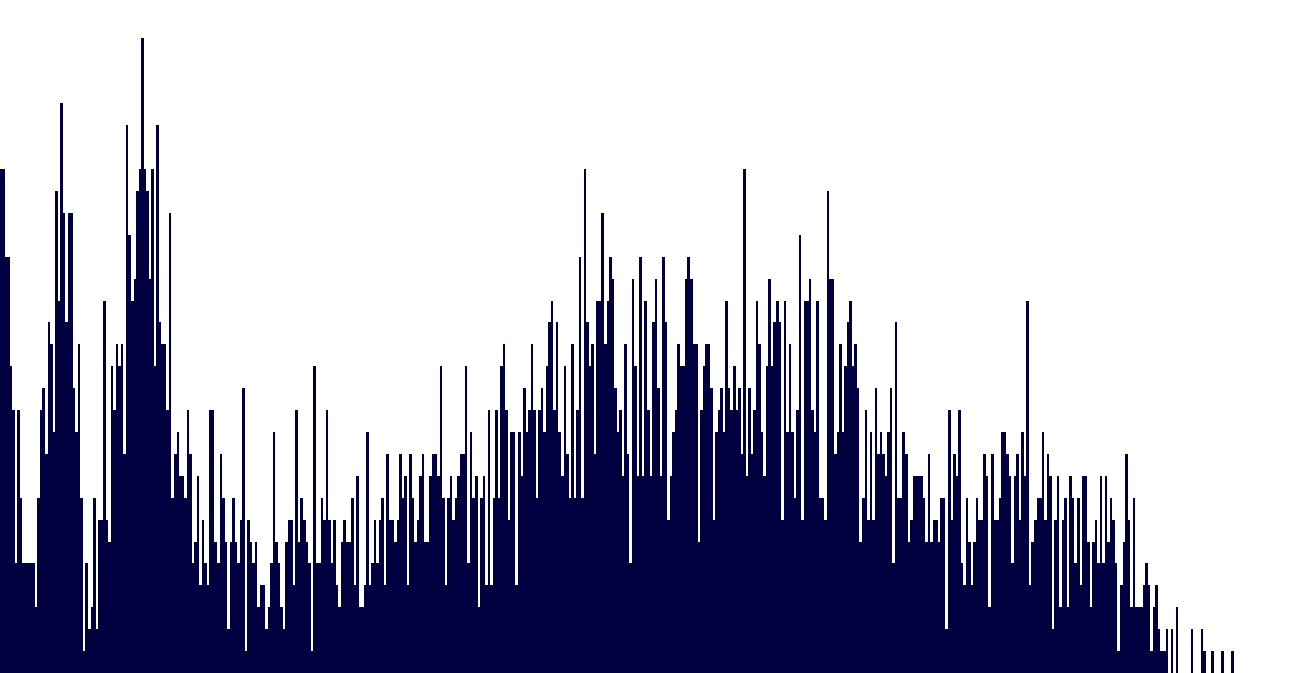
\includegraphics[
%		height=8\baselineskip,
%		width=.8\linewidth,
%		frame
%	]{data/bg_white.png}
%
%	\begin{table}[!h]
%	\vspace{0\baselineskip}
%	\caption[峰值道址]{参考穆斯堡尔谱的峰值道址}
%	\footnotesize
%	\textit{\tup{(1)} \FeAlpha}\\[1ex]
%	\begin{tabularx}{.85\linewidth}{%
%		C{1} | *6{C{.5}}
%	}
%	\toprule\midrule
%		序号 &
%			1 & 2 & 3 & 4 & 5 & 6 \\
%	\midrule
%		右侧峰道址$v_R$ &
%			289 & 327 & 367 & 396 & 436 & 475 \\
%		左侧峰道址$v_L$ &
%			226 & 186 & 147 & 117 & 77 & 38 \\
%	\midrule\bottomrule
%	\end{tabularx}
%	\label{tab:}
%	\vspace{-.3\baselineskip}
%	\end{table}%
\vspace{-.8\baselineskip}
\section{结论}
\vspace{-.5\baselineskip}
%%%	首先要给出实验结果,然后再给出由实验结果分析得到的结果和结论。此部分给出的内容要比摘要中的全面,用词要更准确。\par
%%%%%%%%%%%%%%%%%%%%%%%%%%%%%%%	
	本实验通过考察耗散结构的经典实例:Rayleigh–Bénard对流斑图;实验中比较了$d = \SI{2}{\mm}, \SI{4}{\mm}$薄层去离子水的上下表面温差,观察分析了斑图形成至崩溃的过程,认识并检验了耗散结构的基本特征,初步了解了非线性动力学的分析手段。
\vspace{-.8\baselineskip}
\section{致谢}
\vspace{-.5\baselineskip}
%	此部分感谢同组人...和对实验和报告有帮助的人。
%%%%%%%%%%%%%%%%%%%%%%%%%%%%%%
	感谢周路群老师的细致指导,尤其是老师关于耗散结构和非线性动力学的讲解对本人带来了很大启发;感谢合作者黄江天同学的工作和帮助。
%	感谢 \TeX\, - \LaTeX\, Stack Exchange\footnote{%
%		\url{https://tex.stackexchange.com/}
%	}, 助我解决了众多排版问题。
\vspace{.5\baselineskip}

\setlength{\bibsep}{1ex}
\linespread{1.}\selectfont
\bibliographystyle{../BibStyle/gbt-7714-2015-numerical}
%\bibliographystyle{apsrev4-1}
\bibliography{../BibStyle/Textbook,bib/Ref}
\clearpage
\linespread{1.5}\selectfont
\end{document}